\documentclass{mini}
\usepackage[utf8]{inputenc}
\usepackage[polish]{babel}
\usepackage{enumitem}
\usepackage{todonotes}
\presetkeys
	{todonotes}
	{inline}{}
\usepackage{listings}
\usepackage[lighttt]{lmodern}
\usepackage{xcolor}
\lstset{
    backgroundcolor=\color{yellow!20},%
    basicstyle=\small\ttfamily,%
    numbers=left, numberstyle=\color{gray}\tiny, stepnumber=1
}
\lstset{keywords={%  
		ACS,  after,  always, at, causes, ever,
		generally,  if, imposible,  initially,  
		invokes,  involved, -,  OBS,  perfomed,
		releases, triggers, typically,  when
    },keywordstyle={\bfseries},
    frame=single,
    breaklines=true,
    postbreak=\raisebox{0ex}[0ex][0ex]{\ensuremath{\color{red}\hookrightarrow\space}}
}  

%------------------------------------------------------------------------------%
\title{Scenariusze działań z efektami domyślnymi}
\pm{Tomasz Janiszewski}
\author{Tomasz Janiszewski
\\Jakub Dutkowski
\\Tomasz Łącki
\\Rafał Wyka
\\Maciej Bednarz}
\monthyear{\today}
%------------------------------------------------------------------------------%

\begin{document}
\maketitle
\tableofcontents

\newpage

\section{Opis zadania}
Zadaniem projektu jest opracowanie i zaimplementowanie:
\begin{itemize}
\item języka akcji pewnej klasy systemów dynamicznych,
\item języka kwerend, zapewniającego uzyskanie odpowiedzi na określone pytania.
\end{itemize}
Szczegółowy opis klasy systemów dynamicznych oraz języka akcji jest opisany w rozdziale \ref{sc:jezyk_akcji},
natomiast język kwerend oraz zadawane pytania znajdują się w rozdziale \ref{sc:kwerendy}.
W tym dokumencie znajdują się również przykłady.
Pokazują one konkretne przypadki użycia oraz oczekiwane wyniki działania programu.

\section{Język akcji}\label{sc:jezyk_akcji}

Poniższy język został zaprojektowany tak aby spełnić następujące warunki:
\begin{itemize}
	\item Prawo inercji
	\item Linowy model czasu (czas dyskretny)
	\item Sekwencyjność działań
	\item Niedeterminizm
	\item Z każdą akcją związane są
		\begin{itemize}
			\item Warunki początkowe
			\item Skutki:
				\begin{description}
					\item[środowiskowe] występują natychmiast po zakończeniu akcji
						\begin{description}
							\item[pewne] występuje zawsze po zakończeniu akcji
							\item[typowe] występują zazwyczaj po zakończeniu akcji
						\end{description}
					\item[dynamiczne] występują po czasie $d \geqslant 0$
						\begin{description}
							\item[pewne] występuje zawsze po zakończeniu akcji
							\item[typowe] występują zazwyczaj po zakończeniu akcji
						\end{description}
				\end{description}
			\item Wykonawca (agent)
			\item Czas trwania $t = 1$
		\end{itemize}
	\item Pewne stany mogą rozpoczynać wykonywanie pewnych akcji
	\item Agenci mogą nie potrafić wykonać akcji w pewnych stanach. Stany te są określone przez podanie
	warunków lub konkretnych punktów czasowych.
\end{itemize}
Językiem odpowiadającym powyższym warunkom jest język $\mathcal{AL}$
opisujący dziedzinę akcji z czasem liniowym.

\subsection{Opis symboli języka}
\begin{definition}
Język definiujemy jako trójkę
\begin{equation}
\psi = \left( \mathcal{F}, \mathcal{A}, \mathcal{T} \right)
\end{equation}
\begin{itemize}
\item[$\mathcal{F}$] niepusty zbiór inercji (dalej \emph{fluenty})
\item[$\mathcal{A}$] niepusty zbiór akcji (dalej \emph{akcje}),
$\mathcal{A} = \left\lbrace (\Lambda, \tau) : \Lambda \in \textbf{Agents}, \tau \in \textbf{Tasks} \right\rbrace$
\item[$\mathcal{T}$] niepusty zbiór punktów czasu, $\mathcal{T} = \mathbb{N}$
\end{itemize}
\end{definition}

\subsection{Syntaktyka języka}
\begin{description}[style=nextline]
	\item[$\texttt{initially } \alpha$]
	stan początkowy fluentów w formule $\alpha$
	\item[$a_i \texttt{ causes } \alpha \texttt{ if } \pi$]
	akcja $a_i$\footnote{akcja $a_i$ złożona jest z agenta ($\Lambda$) i zadania ($\tau$), które wykonuje}
	powoduje przejście w stan $\alpha$ jeśli zachodzi warunek $\pi$
	\item[$\texttt{typically } a_i \texttt{ causes } \alpha \texttt{ if } \pi$]
	zazwyczaj akcja $a_i$ powoduje przejście w stan $\alpha$ jeśli zachodzi warunek $\pi$
	\item[$a_i \texttt{ invokes } a_j \texttt{ after } d \texttt{ if } \pi$]
	akcja $a_i$ powoduje wykonanie akcji $a_j$ po $d$ chwilach od zakończenia akcji $a_i$,
	jeśli zachodzi warunek $\pi$
	\item[$\texttt{typically } a_i \texttt{ invokes } a_j \texttt{ after } d \texttt{ if } \pi$]
	zazwyczaj akcja $a_i$ powoduje wykonanie akcji $a_j$ po $d$ chwilach od zakończenia akcji $a_i$,
	jeśli zachodzi warunek $\pi$
	\item[$a_i \texttt{ releases } f \texttt{ after } d \texttt{ if } \pi$]
	akcja $a_i$ powoduje uwolnienie fluentu $f$ po $d$ chwilach od zakończenia akcji $a_i$,
	jeśli zachodzi warunek $\pi$
	\item[$\texttt{typically } a_i \texttt{ releases } f \texttt{ after } d \texttt{ if } \pi$]
	zazwyczaj akcja $a_i$ powoduje uwolnienie fluentu $f$ po $d$ chwilach od zakończenia akcji $a_i$,
	jeśli zachodzi warunek $\pi$
	\item[$\pi \texttt{ triggers } a_i$]
	jeśli zachodzi warunek $\pi$	to wykonywana jest akcja $a_i$
	\item[$\texttt{typically }\pi \texttt{ triggers } a_i$]
	zazwyczaj jeśli zachodzi warunek $\pi$ to wykonywana jest akcja $a_i$
	\item[$\texttt{impossible } a_i \texttt{ at } t \texttt{ if } \pi$]
	akcja $a_i$ jest niemożliwa  w chwili $t$, jeśli zachodzi warunek $\pi$
	\item[$\texttt{always } \pi$]
	każdy stan spełnia warunek $\pi$
\end{description}

\begin{example}\label{przyk:syntaktyka_jezyka_akcji}
Na początku Adam jest głodny, nie ma biletu do kina, jest w domu (zatem nie jest w kinie) i seans kinowy nie jest gotowy (nie można jeszcze wchodzić na salę kinową). 
Warto zwrócić uwagę na fakt, iż zazwyczaj Adam nie mając biletu i będąc w domu, kupi go poprzez internet. 
Jednakże będąc głodnym w czasie 0 zje posiłek, zaś na czas 1 przypada mycie zębów. 
W czasie 2 z kolei Adam musi wyjść do kina. 
Zatem akcja typowa nie wykona się ani razu, mimo iż wszelkie jej warunki w czasie 0, 1 i 2 są spełnione. 
Następnie w czasie 3 Adam typowo kupi bilet będąc w kinie, po czym w czasie 4, również typowo, zacznie oglądać film.

	\begin{lstlisting}
initially hungry, -hasTicket, atHome, -atCinema, -isMovieAvailable
hungry triggers Adam Eat
Adam Eat causes -hungry
Adam WashTeeth at 1
typically -hasTicket and atHome triggers Adam BuyTicketByTheInternet
Adam BuyTicketByTheInternet causes hasTicket if atHome
Adam GoToTheCinema at 2
Adam GoToTheCinema causes -atHome, atCinema
typically atCinema and -hasTicket triggers Adam BuyTicketAtTheCinema
Adam BuyTicketAtTheCinema causes hasTicket if atCinema, -hasTicket
isMovieAvailable at 3
-isMovieAvailable at 5
hasTicket and isMovieAvailable typically causes Adam WatchMovie
	\end{lstlisting}
\end{example}


\subsection{Scenariusze działań}
\begin{definition}
Scenariusze działań definiujemy jako zbiór obserwacji i akcji:
\begin{equation}
	Sc = (OBS, ACS)\\
\end{equation}
\begin{description}
	\item[$OBS = \lbrace(\gamma_1, t_1), \dots, (\gamma_m, t_m)\rbrace$]
	obserwacja, każda obserwacja jest stanem spełniającym warunek $\gamma$ w pewnej chwili $t$
	\item[$ACS = \lbrace(a_1, t_1), \dots, (a_n, t_n) \rbrace$]
	gdzie $a_i$ -- akcje, $t_i$ -- punkt w czasie rozpoczęcia akcji
\end{description}
\end{definition}

\subsection{Semantyka}
\begin{definition}
Semantyczną strukturą języka $\mathcal{AL}$ nazywamy system $ S=(H,O,E,N,T_{\infty }) $ taki, że:
	\begin{itemize}
		\item $ H: Forms(\mathcal{F}) $ $\times$ $ \mathcal{T}$ $\longrightarrow$ $\{0,1\}$ jest funkcją historii,
		pozwala ona stwierdzić, jaki stan ma pewny fluent lub czy dana formuła jest spełniona, dla określonej chwili czasu $t$.
		\item $ O: \mathcal{A}$ $\times$ $ \mathcal{T}$ $\longrightarrow$ $2^{\mathcal{F}}$ jest funkcją okluzji.
		Dla pewnej ustalonej akcji $a_i \in \mathcal{A}$, chwili czasu $t\in\mathbb{N}$, funkcja $O(a_i,t) $ zwraca zbiór
		fluentów, na który akcja $a_i$ ma wpływ, jeśli będzie ona trwała w chwili $t$.
Wartość funkcji okluzji będziemy nazywać regionem okluzji.
		\item $E\subseteq \mathcal{A} \times \mathcal{T}$ jest relacją wykonań akcji. Dwójka $(a_i,t)$ należy do relacji
		$E$ jeśli akcja $a_i$ trwająca jednostkę czasu jest rozpoczęta w czasie t. W naszym modelu zakładamy warunek
		sekwencyjności działań. Oznacza on, że w danym czasie możemy wykonać tylko jedną akcje, tak więc jeśli
		$(a_i, t_1) \in E \land (a_j, t_2) \in E \implies t_1 \neq t_2 \lor a_i = a_j$.
		\item $N\subseteq \mathcal{A} \times \mathcal{T}$ jest relacją typowości\footnote{ang. \emph{normality relation}}.
		Dwójka $(a_i,t)$ należy do relacji $N$, jeśli w chwili $t$ dany stan jest typowy dla akcji $a_i$.
		\item $T_{\infty } \in \mathcal{T} $ jest czasem zakończenia scenariusza, może to być dowolnie duża ustalona liczba naturalna.
		Wielkość ta informuje o tym, do kiedy powinny być zakończone wszystkie akcje w danym scenariuszu.
		Stąd scenariusze nieskończone nie będą rozpatrywane.
	\end{itemize}
\end{definition}

Niech: $a_i,a_j$ będą akcjami, $ f $ - fluentem, $\alpha, \pi$ - formułami, a $fl(\alpha)$ zbiorem fluentów
występujących w $\alpha$. Wtedy dla zdań języka $\mathcal{AL}$  muszą być spełnione następujące warunki:
   \begin{itemize}
   		\item Dla każdego wyrażenia $ ( a_i\;causes\;\alpha\;if\;\pi)\in D $ i dla każdego momentu w czasie
   		$t \in \mathcal{T}$, jeżeli $H(\pi,t)=1$ oraz $(a_i,t) \in E$, wtedy $H(\alpha,t + 1)=1$ mamy $fl(\alpha)\subseteq O(a_i,t + 1)$.
		\item Dla każdego wyrażenia $ ( typically\; a_i\;causes\;\alpha\;if\;\pi)\in D $ i dla każdego momentu w czasie
		 $t \in \mathcal{T}$, jeżeli $H(\pi,t)=1$ oraz $(a_i,t) \in E$, $(a_i,t) \in N$, wtedy $H(\alpha,t + 1)=1$ mamy $fl(\alpha)\subseteq O(a_i,t + 1)$.
 		\item Dla każdego wyrażenia $( a_i\;invokes\;a_j\;after\;d\;\;if\;\pi)\in D$ i dla każdego momentu czasu
 		$t \in \mathcal{T}$, jeżeli $H(\pi,t)=1$, $(a_i,t)\in E $ oraz $t+1+d\leq T_{\infty}$, wtedy $(a_j,t+1+d) \in E $.
	 	\item Dla każdego wyrażenia $( typically\; a_i\;invokes\;a_j\;after\;d\;\;if\;\pi)\in D$ i dla każdego momentu czasu
	 	$t \in \mathcal{T}$, jeżeli $H(\pi,t)=1$, $(a_i,t)\in E$, $(a_j, t + d)\in N $ oraz $t+1+d\leq T_{\infty}$, wtedy $(a_j,t+1+d) \in E $.
   		\item Dla każdego wyrażenia $( a_i\;releases\;f\;if\;\pi)\in D $ i dla każdego momentu czasu
   		$t \in \mathcal{T}$, jeżeli $H(\pi,t)=1$ oraz $(a_i,t)\in E$, wtedy mamy $f\in O(a_i,t+1)$.
 		\item Dla każdego wyrażenia $( typically\; a_i \;releases\;f\;if\;\pi)\in D $ i dla każdego momentu czasu
 		$t \in \mathcal{T}$, jeżeli $H(\pi,t)=1$ oraz $(a_i,t)\in E$ i $(a_i,t)\in N$, wtedy mamy $f\in O(a_i,t+1)$.
   		\item Dla każdego wyrażenia $(\pi\;triggers\; a_i)\in D$ i dla każdego momentu czasu $t \in \mathcal{T}$,
   		jeżeli $H(\pi,t)=1$ oraz $t+1\leq T_{\infty}$, wtedy $(a_i,t)\in E$.
		\item Dla każdego wyrażenia $(typically\; \pi\;triggers\; a_i)\in D$ i dla każdego momentu czasu
		$t \in \mathcal{T}$, jeżeli $H(\pi,t)=1$, $(a_i, t)\in N$ oraz $t+1\leq T_{\infty}$, wtedy $(a_i,t)\in E$.
		\item Dla każdego wyrażenia $(impossible \; a_i \; if\;  \pi )$ i dla każdego momentu czasu $t \in \mathcal{T}$,
		jeżeli $H(\pi,t)=1$, wtedy $(a_i,t) \notin E $.
		\item Dla każdego wyrażenia $(always \; \pi )$ i dla każdego momentu czasu $t \in \mathcal{T}$, $H(\pi,t)=1$.
   \end{itemize}
   \begin{definition}
   Niech $S = (H,O,E,N,T_{\infty})$ będzie strukturą języka $\mathcal{AL}$ , $ Sc=(OBS,ACS) $ będzie scenariuszem,
    oraz $ D $ dziedziną. Powiemy, że $ S $ jest strukturą dla $Sc$ zgodną z opisem dziedziny $D$, jeśli:
   		\begin{itemize}
     		\item Dla każdej obserwacji $(\alpha,t )\in OBS$ mamy $H(\alpha,t )=1$
     		\item $ACS \subseteq E$
     		\item Dla każdej akcji $ {a_i \in \mathcal{A}}$ oraz dla każdego czasu rozpoczęcia akcji
     		$t \in \mathcal{T}$, jeżeli $(a_i,t) \in E $, to $t+1 \leq T_{\infty}$.
    		\end{itemize}
   \end{definition}
   \begin{definition}
	   Niech $O_{1}$,$O_{2}$: $X \longrightarrow 2^{Y}$. Mówimy, że $O_{1} \prec O_{2}$ jeżeli
	   $\forall x\in X$ $O_{1}(x)\subseteq O_{2}(x)$ oraz $O_{1}\neq O_{2}$.
   \end{definition}

   \begin{definition}
   Niech $S=(H,O,E,N,T_{\infty})$ będzie strukturą dla scenariusza $Sc=(OBS,ACS)$ zgodną z opisem dziedziny
   $D$. Mówimy, że $S$ jest $O$-minimalną strukturą, jeżeli nie istnieje struktura \\$S'=(H',O',E',N',T_{\infty}')$
   dla tego samego scenariusza i dziedziny taka, że $H'=H$, $E'=E$ oraz $O'\prec O$.
   \end{definition}
   \begin{definition}
   Niech $S=(H,O,E,N,T_{\infty})$ będzie strukturą dla scenariusza $Sc=(OBS,ACS)$ zgodną z opisem dziedziny
   $D$. $S$ będziemy nazywać modelem typu 1 dla scenariusza $Sc$ zgodnym z opisem $D$ jeżeli:
   \begin{itemize}
		\item $S$ jest $O$-minimalny
		\item Dla każdego momentu w czasie $t \in \mathcal{T}$,  \{$f\in F$: $H(f,t)\neq H(f,t+1) $\}
		$\subseteq O(a_i,t+1)$ dla pewnej akcji $a_i$.
		\item Nie istnieje żadna struktura $S'=(H',O',E',N',T_{\infty}')$ dla $Sc$ zgodna z opisem $D$,
		która spełnia poprzednie warunki oraz taka, że $E'\subset E$.
	\end{itemize}
\end{definition}
\begin{definition}
   Niech $S=(H,O,E,N,T_{\infty})$ będzie strukturą dla scenariusza $Sc=(OBS,ACS)$ zgodną z opisem dziedziny
   $D$. $S$ będziemy nazywać modelem typu 2 dla scenariusza $Sc$ zgodnym z opisem $D$ jeżeli:
   \begin{itemize}
		\item $S$ jest modelem typu 1 dla scenariusza $Sc$
		\item Nie istnieje żaden model $S'=(H',O',E',N',T_{\infty}')$ dla scenariusza $Sc$ taki, że $N \subset N'$.
   \end{itemize}
\end{definition}

\begin{remark}
Zbiór wszystkich modeli typu 1 (odp. typu 2) dla scenariusza $Sc$ oznaczać będziemy przez $Mod1(D, Sc)$ ($Mod2(D, Sc)$).
\end{remark}

\begin{remark}
Nie dla każdego scenariusza można ułożyć model. Mówimy, że scenariusz $Sc$ jest \textit{zgodny}
jeśli istnieje do niego model zgodny z dziedziną $D$.
\end{remark}

\section{Język zapytań}\label{sc:kwerendy}
Zdefiniowany język akcji może być odpytywany przez poniższy język zapytań,
który zwraca odpowiedzi \texttt{TRUE/FALSE} na następujące pytania
\begin{description}[style=nextline]
	\item[Czy w chwili $t$ realizacji scenariusza $Sc$ warunek $\gamma$ zachodzi zawsze/kiedykolwiek/na ogół?]
	$\texttt{always/ever/typically } \gamma \texttt{ at } t \texttt{ when } Sc$
	\item[Czy w chwili $t$ realizacji scenariusza $Sc$ akcja $a$ wykonywana jest zawsze/kiedykolwiek?]
	$\texttt{always/ever/typically performed } a_i \texttt{ at } t \texttt{ when } Sc$
	\item[Czy realizacji scenariusza $Sc$ zaangażowana jest grupa agentów $Ag$ zawsze/kiedykolwiek?]
	$\texttt{always/ever involved } Ag \texttt{ when } Sc$
\end{description}

\subsection{Przykłady}

\begin{example}
Rozważmy system opisany w przykładzie \ref{przyk:syntaktyka_jezyka_akcji}.
Oznaczenia fluentów: hungry (h), hasTicket (t), atHome (ah), atCinema (ac), isMovieAvailable (m)

\begin{figure}[h!]
	\centering
	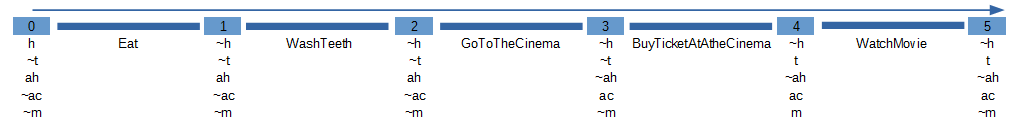
\includegraphics[width=1\textwidth]{example1_1}
	\caption{Diagram dla scenariusza $Sc$}
	\label{PicSC1}
\end{figure}

Rozważmy, co będzie, gdy z powyższego opisu języka akcji i scenariusza usuniemy dwa zdania:

	\begin{lstlisting}
hungry triggers Adam Eat
Adam WashTeeth at 1
	\end{lstlisting}

a zamiast nich wstawimy

	\begin{lstlisting}
typically hungry triggers Adam Eat
typically Adam Eat invokes Adam WashTeeth in 1 
BuyPopcorn occurs at 3
	\end{lstlisting}
	
Wówczas otrzymamy trzy modele. 
Adam albo zje, ale nie zdąży umyć zębów, co będzie zachowaniem nietypowym. 
Albo Adam nie zje, co również będzie zachowaniem nietypowym. 
Należy zwrócić uwagę, iż we wszystkich przypadkach Adam ma czas na kupienie biletu z domu przez internet. 

\begin{figure}[h!]
	\centering
	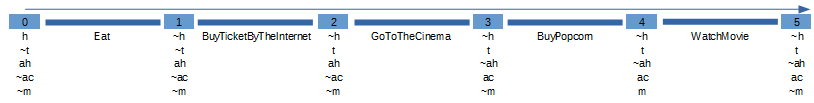
\includegraphics[width=1\textwidth]{example1_2model1}
	\caption{Diagram dla scenariusza $Sc$}
	\label{PicSC2}
\end{figure}

\begin{figure}[h!]
	\centering
	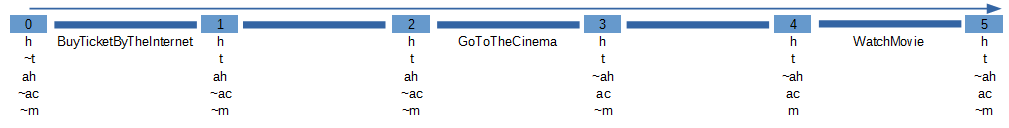
\includegraphics[width=1\textwidth]{example1_2model2}
	\caption{Diagram dla scenariusza $Sc$}
	\label{PicSC3}
\end{figure}

\begin{figure}[h!]
	\centering
	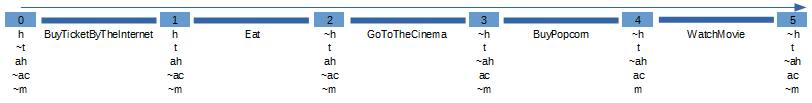
\includegraphics[width=1\textwidth]{example1_2model3}
	\caption{Diagram dla scenariusza $Sc$}
	\label{PicSC4}
\end{figure}

Przykładowe kwerendy dla ostatniego przykładu

	\begin{lstlisting}
always hasTicket at 1
ever hasTicket at 1
	\end{lstlisting}	
powinno zwrócić
	\begin{lstlisting}
FALSE
TRUE
	\end{lstlisting}		
\end{example}	

\begin{example}
Rozważmy przykład studenta Janka. Janek mieszka w akademiku. 
Przed wyjściem zazwyczaj bierze ze sobą kartę wstępu do pokoju i zamyka pokój. 
Janek w chwili 2 wraca do akademika. W chwili 3 dozorca zamyka akademik i nie można do niego wejść. 
Oznaczenia fluentów: roomClosed(r) , hostelClosed(h), inRoom(i), hasCard(c)

	\begin{lstlisting}
initially -roomClosed, -hostelClosed, inRoom, -hasCard
DoorKeeper closeDoor causes hostelClosed
typically -hasCard triggers Janek TakeCard if inRoom
typically Janek Leave invokes Janek LockTheRoom
Janek LockTheRoom causes roomClosed
Janek TakeCard causes hasCard
Janek Leave causes -inRoom
Janek Comeback causes inRoom, -roomClosed if hasCard, roomClosed, -inRoom, -hostelClosed
Janek Comeback causes inRoom if -inHostel, -hostelClosed
typically DoorKepper CloseDoor occurs at 4
Janek Leave occurs at 1
Janek Comeback occurs at 3
	\end{lstlisting}

\begin{figure}[h!]
	\centering
	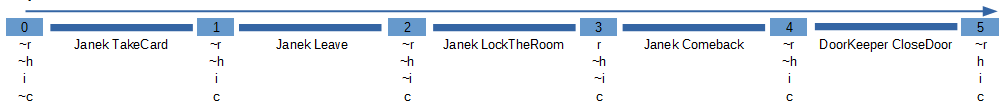
\includegraphics[width=1\textwidth]{example2}
	\caption{Diagram dla scenariusza $Sc$}
	\label{PicSC5}
\end{figure}
\end{example}

\subsection{Semantyka}
Niech $Sc$ będzie scenariuszem, a $D$ opisem dziedziny języka. Powiemy, że kwerenda $Q$ jest konsekwencją
$Sc$ zgodnie z $D$ (ozn. $Sc,\ D\ |\approx\ Q $)

\begin{itemize}
	\item zapytanie kwerendą $Q$ postaci $\gamma\ \texttt{at}\ t\ \texttt{when}\ Sc$\\ zwróci wynik $TRUE$, jeśli\\
	\begin{description}
		\item[always] $\forall_{S=(H,O,E,N,T_{\infty}) \in Mod1(D, Sc)}\; H(\gamma,t)=1$
		\item[ever] $\exists_{S=(H,O,E,N,T_{\infty}) \in Mod1(D, Sc)}\; H(\gamma,t)=1$
		\item[typically] $\forall_{S=(H,O,E,N,T_{\infty}) \in Mod2(D, Sc)}\; (a_i, t) \in N \implies H(\gamma,t)=1$
	\end{description}
	\item zapytanie kwerendą $Q$ postaci $\texttt{performed}\ a_i\ \texttt{at}\ t\ \texttt{when}\ Sc$\\
	zwróci wynik $TRUE$, jeśli
	\begin{description}
		\item[always] $\forall_{S=(H,O,E,N,T_{\infty}) \in Mod1(D, Sc)}\; (a_i,t) \in E$
		\item[ever] $\exists_{S=(H,O,E,N,T_{\infty}) \in Mod1(D, Sc)}\; (a_i,t) \in E$
		\item[typically] $\forall_{S=(H,O,E,N,T_{\infty}) \in Mod2(D, Sc)}\; (a_i,t) \in N \implies (a_i,t) \in E$
	\end{description}
	\item zapytanie kwerendą $Q$ postaci $\texttt{involved}\ \Lambda \; \texttt{when}\ Sc$\\ zwróci wynik $TRUE$, jeśli
	\begin{description}
		\item[always] $\forall_{S=(H,O,E,N,T_{\infty}) \in Mod1(D, Sc)}\; \exists_{((\Lambda', \tau), time) \in N} ((\Lambda', \tau),t) \in E, \Lambda' = \Lambda$
		\item[ever] $\exists_{S=(H,O,E,N,T_{\infty}) \in Mod1(D, Sc)}\; \exists_{((\Lambda', \tau),t) \in E} \Lambda' = \Lambda$
	\end{description}
\end{itemize}

\begin{remark}
   Jeśli warunek nie zajdzie program zwróci wartość $FALSE$.
\end{remark}
\section{Gramatyka}
\lstinputlisting{../src/main/antlr/ActionLanguage.g4}

\begin{example}~\\
\lstinputlisting{../src/test/resources/example_2.1.al}
\end{example}

\end{document}
